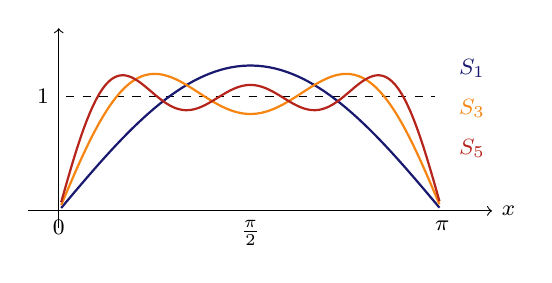
\begin{tikzpicture}[x=1.55cm,y=1.45cm,every node/.style={font=\footnotesize}]
  \draw[black,dashed] (0.06,1)--(3.08,1);
  \draw[MidnightBlue,thick] plot[domain=0.02:3.12,samples=70] (\x,{4/pi*sin((\x) r)});
  \draw[BurntOrange,thick] plot[domain=0.02:3.12,samples=90] (\x,{4/pi*(sin((\x) r)+sin((3*\x) r)/3)});
  \draw[BrickRed,thick] plot[domain=0.02:3.12,samples=120] (\x,{4/pi*(sin((\x) r)+sin((3*\x) r)/3+sin((5*\x) r)/5)});
  \draw[->] (-0.25,0)--(3.55,0) node[right] {$x$};
  \draw[->] (0,-0.15)--(0,1.6);
  \node[below] at (0,0) {$0$};
  \node[below] at (1.5708,0) {$\frac\pi2$};
  \node[below] at (3.1416,0) {$\pi$};
  \node[left] at (0,1) {$1$};
  \node[MidnightBlue,anchor=west] at (3.2,1.25) {$S_1$};
  \node[BurntOrange,anchor=west] at (3.2,0.9) {$S_3$};
  \node[BrickRed,anchor=west] at (3.2,0.55) {$S_5$};
\end{tikzpicture}
